\documentclass[12pt]{article}

\usepackage[portuguese]{babel}
\usepackage{graphicx}
\usepackage{float}

\usepackage{indentfirst}

\usepackage{geometry}

\geometry{
	paper=a4paper,
	margin=60pt
}

\author{
	Felipe Scherer Vicentin\\
	248283
	\and
	Gustavo Miller Santos\\
	248320
}

\title{Diagrama de Processo}

\begin{document}

\maketitle

\section*{Visão geral do diagrama}

\begin{figure}[H]
	\centering
	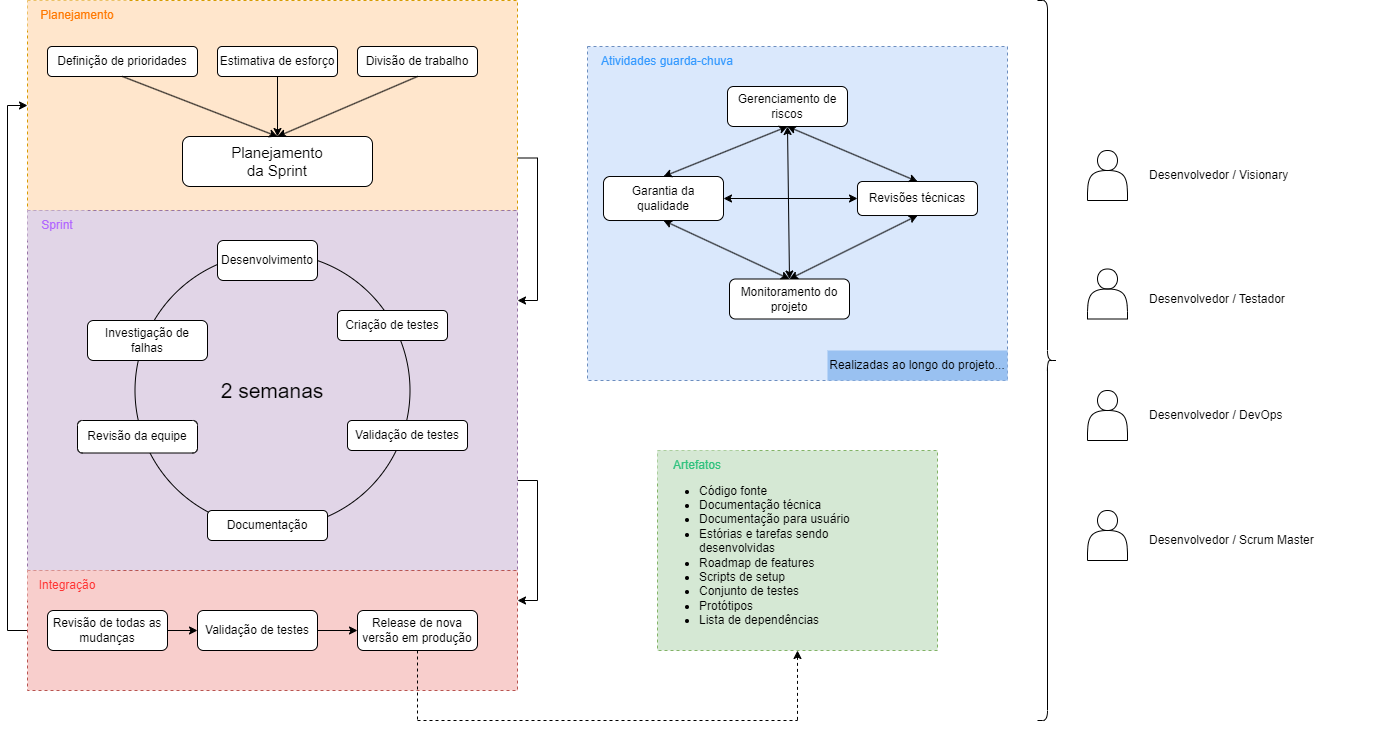
\includegraphics[width=\linewidth]{images/process_diagram.png}
\end{figure}

\section*{Explicação textual}

O processo foi dividido em planejamento, atuação cíclica (sprint), atuação constante (atividades guarda-chuva), e integração.
A ideia foi de manter um processo cíclico com iterações curtas (duas semanas), para incentivar entregas e replanejamentos frequentes.
Aqui, partimos do pressuposto que o processo seria utilizado em um projeto como o da matéria de MC426, e portanto a equipe é responsável por todas as etapas: especificação, desenvolvimento, validação e evolução.

\subsection*{Processo base}

O processo foi baseado na metodologia SCRUM:\@ iterações curtas, com uma fase de planejamento, uma de desenvolvimento, e uma de integração a cada ciclo.
Cada iteração consistirá de 2 semanas.

Similarmente ao SCRUM, o backlog é atualizado frequentemente independente dos ciclos.
No entanto, o planejamento foi simplificado para incluir o refinamento (detalhamento e estimativa de esforço), seguido de priorização, definição do que entra no ciclo seguinte, e por fim divisão de trabalho.

Feito isso, temos a sprint em si que consiste em desenvolvimento, criação e validação de testes, documentação, revisão da equipe e investigação de falhas.

Uma vez que a sprint chega ao fim, temos a etapa de integração: as mudanças são revisadas, os testes são executados, e é feita a release em produção.

\subsection*{Atividades fundamentais e guarda-chuva}

As quatro atividades fundamentais foram descritas acima. São elas:

\begin{itemize}
	\item \textbf{Especificação}: o backlog é atualizado constantemente à medida que a equipe interage para definir sua visão de longo prazo. Esse backlog é refinado na etapa de planejamento, momento em que são definidos os pormenores.
	\item \textbf{Desenvolvimento}: acontece dentro da sprint, e inclui a criação dos testes para garantia de qualidade do que foi desenvolvido.
	\item \textbf{Validação}: além dos testes, a equipe faz uma validação de cada feature a ser entregue. E ao final do ciclo, há novamente uma validação em conjunto.
	\item \textbf{Evolução}: a qualquer momento, as especificações podem ser alteradas pela equipe ou um \textit{bug} grave pode ser encontrado. Se isso acontecer, o backlog é atualizado, e as atividades serão repriorizadas para a sprint seguinte.
\end{itemize}

\subsection*{Principais artefatos}


\subsection*{Papéis dos envolvidos no processo}


\end{document}
